\subsection{Large Oscillations; Energy Aperture}\label{sec:3.6}

A storage ring guide field can usually accept only a small range of energies -- typically
 only a few percent of the nominal energy -- and the magnetic focusing forces are usually reasonably linear over the whole energy range. Even much smaller energy deviations however, may correspond to rather large oscillations of the time displacement $\tau$. I mean by ``large'' oscillations those for which $V(\tau)$ departs significantly from a linear dependence on $\tau$.
 Such large amplitudes may typically occur when the peak rf voltage is not very much larger than the radiation loss (as is usually the case at very high energies) or when the rf harmonic number
$k$ is very large. We should take at least a brief look at the large amplitude oscillations  because they are generally responsible for determining the energy “aperture” -- or “acceptance”
 -- of a ring. Please keep in mind however, that although we shall be dealing with ``large'' time displacements -- which may encompass a major fraction of an rf period - the maximum energy deviations will still be ``small'', a very small fraction of the energy itself.\\
We may begin with the two basic results of the preceding section, Eqs.~\eqref{eq:3.32} and \eqref{eq:3.34}. As before, we replace $U_{\text{rad}}$ by $U_0 + D\epsilon$, since the energy deviations remain small. But we must retain $V(\tau)$ without any simplification. We get for
Eq.~\eqref{eq:3.34}
\begin{align}
	\dfrac{d\epsilon}{dt} = \dfrac{eV(\tau)-U_0}{T_0}-\dfrac{D\epsilon}{T_0}.
\end{align}
If we now express both $\epsilon$ and its time derivative in terms of $\tau$ by using Eq.~\eqref{eq:3.32} we get the following equation.
\begin{align}\label{eq:3.49}
	\dfrac{d^2\tau}{dt^2} = -\dfrac{\alpha}{E_0 T_0} \left\lbrace eV(\tau) - U_0 \right\rbrace - \dfrac{D}{T_0} \dfrac{d\tau}{dt}.
\end{align}
This equation describes the variation of $\tau$ for all amplitudes.\\
I now ask you to look at another equation which is probably familiar to you:
\begin{align}\label{eq:3.50}
	m\dfrac{d^2x}{dt^2} = F(x) - \mu \dfrac{dx}{dt}.
\end{align}
It represents the motion in one dimension, $x$, of a particle of mass $m$, which
moves in a conservative force field $F(x)$, and suffers a frictional drag force proportional
 to its speed. We can understand Eq.~\eqref{eq:3.49} by making a direct comparison between it and Eq.~\eqref{eq:3.50}. The motion in $\epsilon$ is exactly like the motion of a particle of unit mass which moves in the conservative force field
\begin{align}\label{eq:3.51}
	F(\tau) = - \dfrac{\alpha}{E_0 T_0} \left\lbrace eV(\tau) - U_0 \right\rbrace.
\end{align}
and which is subject to a frictional drag proportional to the velocity with a drag coefficient
 $D/T_0$.\\
 The motion in $\tau$ can, in general, only be evaluated by a numerical computation. We can however, get a good heuristic idea of the motion by considering first what happens if the friction term is zero. It is small anyway and can be taken into account later as a perturbation.
 We wish to study the motion
\begin{align}
	m\dfrac{d^2x}{dt^2} = F(x)
\end{align}
with $F(\tau)$, given by Eq.~\eqref{eq:3.51}. As you know such an equation is often handled by
defining a ``potential energy'' function $\Phi(\tau)$ which is the negative of the integral
 of the force. Let's define
\begin{align} \label{eq:3.53}
	\Phi(\tau) = \dfrac{\alpha}{E_0 T_0} \int_0^\tau \left\lbrace eV(\tau) - U_0 \right\rbrace d\tau.
\end{align}
We can then analyze the motion by evoking the principle of conservation of ``energy''. At each instant the sum of the ``potential energy'' $\Phi(\tau)$ and the ``kinetic energy'' -- here $\frac{1}{2} (d\tau/dt)^2$ -- must be a constant, the ``total energy''. The total energy is
also the maximum $\Phi_0$ that can be reached by $\Phi(\tau)$ -- which will occur when $d\tau/dt$
is zero -- so we may write that
\begin{align}\label{eq:3.54}
	\dfrac{1}{2}\left(\dfrac{d\tau}{dt}\right)^2 = \Phi_0 - \Phi(\tau).
\end{align}
Suppose that the energy gain function $eV(\tau)$ has the form shown in Fig.~\ref{fig:fig36}(a) and that the synchronous energy gain $U_0$ is as shown there. Then $\Phi(\tau)$ will be as drawn in part (b) of the figure. The form shown is quite typical.  Notice that there is a general downward trend of $\Phi(\tau)$ with an average slope of $-U_0$. This must occur because the rf accelerating fields must integrate to zero over each complete cycle (at least over each complete cycle of the lowest frequency present).\\
You can now visualize the nature of the time displacement oscillations. The motion is like that of a point particle (an ``electron'') which slides around ``on'' the hilly surface represented by $\Phi(\tau)$ -- where you must of course, think of $\tau$ as a horizontal spatial coordinate. First, there is a potential minimum at $\tau = 0$. If you place an electron there it remains stationary; it is a ``synchronous electron''\footnote{There are of course, stationary points at each potential minimum and these correspond to the synchronous electrons at the centers of other bunches (so long as $\tau < T_0$)}. It however, you place an electron at $\tau_1$ -- so that it is at point $A$ on the hill -- it will slide down the hill and coast up the other side to point $B$. Both $A$ and $B$ are at the same height $\Phi_0 = \Phi(\tau_A)$. At $\tau_A$ and $\tau_B$
 the ``kinetic energy'' will be zero. The kinetic energy will reach its maximum value as the electron passes $\tau = 0$. At each $\tau$ the kinetic energy is given by Eq.~\eqref{eq:3.54} and from it we can obtain the ``velocity'' at each $\tau$:
\begin{align}
	\dfrac{d\tau}{dt} = \pm \sqrt{2} \left[ \Phi_0 - \Phi(\tau) \right]^{1/2}.
\end{align}
Remember, now, that according to Eq.~\eqref{eq:3.32} the ``velocity'' is
\begin{align*}
	\dfrac{d\tau}{dt} = - \alpha \dfrac{\epsilon}{E_0},
\end{align*}
so that the energy deviation (of the real electron) at each $\tau$ is given by
\begin{align}\label{eq:3.56}
	\dfrac{\epsilon(\tau)}{E_0} = \mp \dfrac{\sqrt{2}}{\alpha} \left[ \Phi_0 - \Phi(\tau) \right]^{1/2}.
\end{align}

\begin{figure}[!htb]
	\centering
	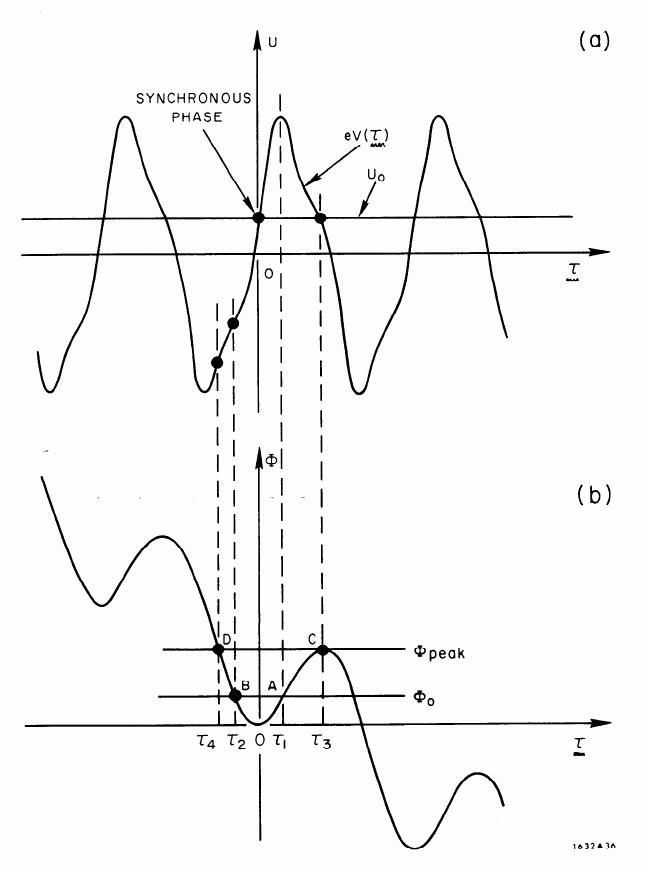
\includegraphics[width=0.8\linewidth]{./Figuras/fig36.jpeg}
	\caption{(a) The rf accelerating function $eV(\tau)$, and (b) the effective potential energy function $\Phi(\tau)$.}
	\label{fig:fig36}
\end{figure}

you can easily see that if you plot a phase diagram -- $\epsilon$ versus $\tau$ -- you will get
a more-or-less elliptical curve much like the curve a drawn in Fig.~\ref{fig:fig37}. You must only use-your common sense to choose the proper sign for the square root on each half cycle.

\begin{figure}[!htb]
	\centering
	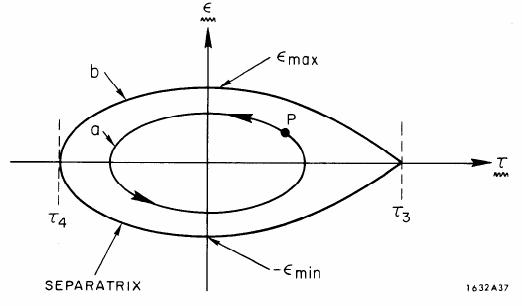
\includegraphics[width=0.8\linewidth]{./Figuras/fig37.jpeg}
	\caption{Phase diagram for large oscillations. Bounded energy oscillations occur only inside of the separatrix.}
	\label{fig:fig37}
\end{figure}

Also you can see what would happen if you were now to include the friction term -- the radiation
 damping. During each oscillation cycle a small amount of energy would be lost in a resulting decrease of the total ``energy'' (You could even estimate this loss by, say, approximating the motion by a sinusoid).\\
It should also be apparent that there will be a maximum amplitude of a stable (periodic) oscillation of $\tau$. It occurs when the electron can just reach the peak of the hill at $\tau_3$ -- corresponding to the point $C$ in Fig.\ref{fig:fig36}(b) - where $\Phi(\tau)$ takes on the value $\Phi_\text{max}$. An electron with any larger amplitude will sail on over the peak
and on into the next valley where it will have so much ``kinetic energy'' that it will keep on going forever -- until it is lost from the storage ring.\\
The maximum stable oscillation goes back and forth between the points $C$ and $D$. Notice that the point $C$ is also where $eV(\tau)$ is again equal to $U_0$. (To the left of $C$ the real electron always gains energy and may have some hope of returning to the origin of $\tau$). The other extreme of the oscillation at point $D$ has no special quality except that $\Phi(\tau)$ is again equal to $\Phi_\text{max}$, the value at $C$. The phase diagram of the extreme oscillation
 is a little peculiar, since both the velocity and the acceleration go to zero at $C$ but not at $D$.  The electron ``lingers'' at $C$ - in the ideal case for an infinite time! As a result the phase diagram will have a ``corner'' as shown by the curve (b) of Fig.~\ref{fig:fig37}. This special curve is called the separatrix, because it separates the stable oscillations from the unstable trajectories. An electron injected into a storage ring with a certain energy deviation $\epsilon$ and time displacement $\tau$ corresponding to the point $P$ in Fig.~\ref{fig:fig37} will circulate on a more-or-less elliptical closed curve (neglecting damping). If an electron is injected at a point outside the separatrix it is ``lost''.\\
 You can now see how the rf system can determine the energy aperture of a storage ring. Energy deviations larger than $\pm\epsilon_\text{max}$ -- of Fig.~\ref{fig:fig37} -- cannot be held in the storage ring. Electrons may be lost at smaller energy deviations if the lateral displacements
 $x_\epsilon$ associated with $\epsilon$ cause the electron to collide with some physical obstruction that limits the radial aperture. Normally, however, the rf limitation sets in first
 and the energy aperture is $\pm\epsilon_\text{peak}$. From Eq.~\eqref{eq:3.56},
\begin{align}
	\dfrac{\epsilon_{\max}}{E_0} = \dfrac{1}{\alpha} (2 \Phi_{\max})^{1/2}.
\end{align}
For the special case of an rf voltage function that is a pure sinusoid -- as described by Eq.~\eqref{eq:3.36} -- it is possible to calculate $\Phi(\tau)$ using Eq.~\eqref{eq:3.53},
\begin{align}\label{eq:Phi_sine}
	\Phi(\tau) = \dfrac{\alpha U_0}{2\pi k E_0} \left\lbrace \sqrt{q^2-1} - q \cos [\omega_{\text{rf}}\tau - \phi_0] - \omega_{\text{rf}} \tau \right\rbrace,
\end{align}
in which
\begin{align} \label{eq:3.60}
q = e\hat{V}/U_0
\end{align}
is the overvoltage -- namely the ratio of the peak rf voltage to the minimum voltage required to store a synchronous electron. Notice that, from Fig.~\ref{fig:fig36}, $\Phi_{\max}$ happens the first time $\Phi'(\tau^*) = 0$ for $\tau^* > 0$. More precisely, we have the next point for which $\sin[\omega_{\text{rf}}\tau^*-\phi_0]$ assumes the same value as $\sin[-\phi_0)]$, that is
\begin{align*}
	& \omega_{\text{rf}}\tau^* - \phi_0 = \pi - (-\phi_0) \\
    \Rightarrow \, & \tau^* = \dfrac{\pi}{\omega_{\text{rf}}} + \dfrac{2\phi_0}{\omega_{\text{rf}}}.
\end{align*}

Plugging this result in Eq.~\eqref{eq:Phi_sine}, results in
\begin{align} \label{eq:3.58}
	\Phi_{\max} = \dfrac{\alpha U_0}{2\pi k E_0} F(q),
\end{align}
where
\begin{align}
	F(q) = 2\left\lbrace \sqrt{q^2 - 1} - \arccos(1/q) \right\rbrace.
\end{align}

The energy aperture $\epsilon_{\max}$ for this case is then given by
\begin{align}
	\left(\dfrac{\epsilon_{\max}}{E_0}\right)^2 = \dfrac{U_0}{\pi \alpha k E_0} F(q).
\end{align}
The aperture function $F(q)$ is plotted in Fig.~\ref{fig:fig38}. Notice that for large $q$
\begin{align}
	F(q) \to 2q - \pi.
\end{align}

\begin{figure}[!htb]
	\centering
	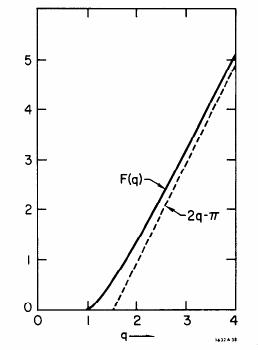
\includegraphics[width=0.5\linewidth]{./Figuras/fig38.jpeg}
	\caption{The energy aperture function F(q).}
	\label{fig:fig38}
\end{figure}

Finally if you think about what happens if you start an electron outside of the energy aperture
 -- say at points above the point D on the curve of $\Phi(\tau)$ in Fig.~\ref{fig:fig36}(b)
and figure out what their phase trajectories will be you will see that they become curves like the ones drawn in Fig.~\ref{fig:fig39}. Three successive separatrices are shown and several examples of unstable trajectories. Again you see that an electron once outside a stable region will -- barring a fortunate accident -- stay outside forever.

\begin{figure}[!htb]
	\centering
	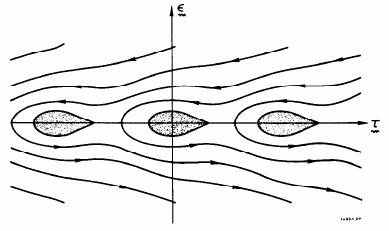
\includegraphics[width=0.8\linewidth]{./Figuras/fig39.jpeg}
	\caption{Phase trajectories for electrons not captured in a bunch (a qualitative sketch).}
	\label{fig:fig39}
\end{figure}
